\subtitle{\bf Aula 5 - Introdu\c{c}\~{a}o}
\begin{frame}[t,plain]
\titlepage
\end{frame}

\begin{frame}{Objetivos}
\protect\hypertarget{objetivos-1}{}
\begin{itemize}
\item
  Motivar o uso de gramáticas livres de contexto para especifica\c{c}\~{a}o da
  estrutura sintática de linguagens.
\item
  Revisar alguns conceitos sobre linguagens livres de contexto.
\item
  Apresentar problemas comuns na modelagem de sintaxe usando gramáticas.
\end{itemize}
\end{frame}

\hypertarget{introduuxe7uxe3o}{%
\section{Introdu\c{c}\~{a}o}\label{introduuxe7uxe3o}}

\begin{frame}{O Papel da Análise Sintática}
\protect\hypertarget{o-papel-da-anuxe1lise-sintuxe1tica}{}
\begin{itemize}

\item
  Após a análise léxica, o programa é uma \textbf{lista de tokens}
\item
  A análise sintática verifica se os tokens formam uma \textbf{estrutura
  válida}
\item
  Produz uma \textbf{Árvore Sintática Abstrata (AST)}
\end{itemize}
\end{frame}

\begin{frame}{O Papel da Análise Sintática}
\protect\hypertarget{o-papel-da-anuxe1lise-sintuxe1tica-1}{}
\begin{itemize}

\item
  N\~{a}o verifica tipos, declara\c{c}\~{o}es de variáveis, etc. (papel da análise
  sem\^{a}ntica)
\item
  A AST é usada pelas fases seguintes do compilador
\end{itemize}
\end{frame}

\begin{frame}{Por que n\~{a}o ERs?}
\protect\hypertarget{por-que-nuxe3o-ers}{}
\begin{itemize}

\item
  Par\^{e}nteses balanceados requerem \textbf{contar} indefinidamente
\item
  Aut\^{o}matos finitos t\^{e}m um número \textbf{fixo} de estados
\item
  Impossível contar número ilimitado de par\^{e}nteses abertos com AFD
\end{itemize}
\end{frame}

\begin{frame}{Por que n\~{a}o ERs?}
\protect\hypertarget{por-que-nuxe3o-ers-1}{}
\begin{itemize}

\item
  Lema do Bombeamento: \(\{a^n b^n \mid n \geq 0\}\) n\~{a}o é regular
\item
  \textbf{Solu\c{c}\~{a}o}: Gramáticas Livres de Contexto (GLCs)
\end{itemize}
\end{frame}



\begin{frame}{Defini\c{c}\~{a}o Formal}
\protect\hypertarget{definiuxe7uxe3o-formal}{}
Uma GLC \(G = (V, \Sigma, R, P)\):

\begin{itemize}

\item
  \(V\): conjunto de \textbf{n\~{a}o-terminais} (variáveis sintáticas)
\item
  \(\Sigma\): conjunto de \textbf{terminais} (tokens)
\item
  \(R\): conjunto de \textbf{produ\c{c}\~{o}es} da forma \(A \to \alpha\)
\item
  \(P \in V\): \textbf{símbolo inicial}
\end{itemize}
\end{frame}

\begin{frame}{Exemplo: Linguagem Exp}
\protect\hypertarget{exemplo-linguagem-exp}{}
\[E \to n \mid E + E \mid E * E \mid (E)\]

\begin{itemize}

\item
  \(\Sigma = \{+, *, (, ), n\}\) s\~{a}o os tokens da linguagem
\item
  \(V = \{E\}\) é o único n\~{a}o-terminal
\item
  Derivamos strings aplicando produ\c{c}\~{o}es repetidamente
\end{itemize}
\end{frame}

\begin{frame}{Deriva\c{c}\~{o}es}
\protect\hypertarget{derivauxe7uxf5es}{}
\begin{itemize}

\item
  Uma string pertence a \(L(G)\) se existe uma \textbf{deriva\c{c}\~{a}o} a
  partir do símbolo inicial:
\end{itemize}

\[
\begin{array}{l}
   E \Rightarrow E+E \Rightarrow \\
  (E)+E \Rightarrow (E+E)+E \Rightarrow \\
  (1+E)+E \Rightarrow (1+4)+E \Rightarrow\\
  (1+4)+2
\end{array}
\]
\end{frame}

\begin{frame}{Deriva\c{c}\~{o}es}
\protect\hypertarget{derivauxe7uxf5es-1}{}
\begin{itemize}

\item
  Cada passo aplica uma produ\c{c}\~{a}o:

  \begin{itemize}

  \item
    Forma sentencial atual: \(\alpha A \beta\)
  \item
    Regra \(A \to \gamma\)
  \item
    Resultado: \(\alpha A \beta \to \alpha \gamma \beta\)
  \end{itemize}
\end{itemize}
\end{frame}

\begin{frame}{Deriva\c{c}\~{o}es}
\protect\hypertarget{derivauxe7uxf5es-2}{}
\begin{itemize}

\item
  \textbf{Deriva\c{c}\~{a}o mais \`{a} esquerda}: expande o n\~{a}o-terminal mais \`{a}
  esquerda
\item
  \textbf{Deriva\c{c}\~{a}o mais \`{a} direita}: expande o mais \`{a} direita
\end{itemize}
\end{frame}

\begin{frame}[fragile]{Exemplo}
\protect\hypertarget{exemplo}{}
\begin{itemize}

\item
  Deriva\c{c}\~{a}o Mais \`{a} Esquerda de \texttt{(1+4)+2}
\end{itemize}

\[\begin{array}{lc}
E     & \Rightarrow \\
E + E & \Rightarrow \\
(E) + E & \Rightarrow \\
(E + E) + E & \Rightarrow \\
(1 + E) + E & \Rightarrow \\
(1 + 4) + E & \Rightarrow \\
(1 + 4) + 2
\end{array}\]
\end{frame}

\begin{frame}[fragile]{Exemplo}
\protect\hypertarget{exemplo-1}{}
\begin{itemize}

\item
  Deriva\c{c}\~{a}o Mais \`{a} Direita de \texttt{(1+4)+2}
\end{itemize}

\[\begin{array}{lc}
E     & \Rightarrow \\
E + E & \Rightarrow \\
E + 2 & \Rightarrow \\
(E) + 2 & \Rightarrow \\
(E + E) + 2 & \Rightarrow \\
(E + 4) + 2 & \Rightarrow \\
(1 + 4) + 2
\end{array}\]

Ambas as deriva\c{c}\~{o}es correspondem \`{a} mesma árvore sintática.
\end{frame}

\hypertarget{ambiguidade}{%
\section{Ambiguidade}\label{ambiguidade}}

\begin{frame}[fragile]{Ambiguidade}
\protect\hypertarget{ambiguidade-1}{}
\begin{itemize}

\item
  Uma gramática é \textbf{ambígua} se alguma string tem \textbf{mais de
  uma árvore sintática}
\item
  A gramática \(E \to n \mid E+E \mid E*E \mid (E)\) é ambígua!
\item
  Para \texttt{2 + 3 * 4}:
\end{itemize}
\end{frame}

\begin{frame}{Duas Árvores}
\protect\hypertarget{duas-uxe1rvores}{}
\begin{itemize}

\item
  Árvore 1: raiz é \(E+E\) → calcula \((2+3)*4 = 20\) (errado!)
\item
  Árvore 2: raiz é \(E*E\) → calcula \(2+(3*4) = 14\) (correto)
\item
  Ambiguidade causa resultados diferentes dependendo da interpreta\c{c}\~{a}o
\end{itemize}
\end{frame}

\begin{frame}{Solu\c{c}\~{a}o}
\protect\hypertarget{soluuxe7uxe3o}{}
\begin{itemize}

\item
  Hierarquia de Preced\^{e}ncia
\end{itemize}

\[\begin{array}{lcl}
E &\to& E + T \mid T \\
T &\to& T * F \mid F \\
F &\to& n \mid (E)
\end{array}\]
\end{frame}

\begin{frame}{Solu\c{c}\~{a}o}
\protect\hypertarget{soluuxe7uxe3o-1}{}
\begin{itemize}

\item
  \(E\) (Express\~{a}o): somas
\item
  \(T\) (Termo): produtos
\item
  \(F\) (Fator): átomos e express\~{o}es parentesadas
\item
  Multiplica\c{c}\~{a}o tem \textbf{maior preced\^{e}ncia} que adi\c{c}\~{a}o
\end{itemize}
\end{frame}

\begin{frame}{Preced\^{e}ncia}
\protect\hypertarget{preceduxeancia}{}
\begin{itemize}

\item
  Express\~{a}o de preced\^{e}ncia \(i+1\)

  \begin{itemize}

  \item
    Associatividade \`{a} direita
  \end{itemize}
\end{itemize}

\[
E_{i + 1} \to E_i \otimes E_{i + 1}
\]
\end{frame}

\begin{frame}{Preced\^{e}ncia}
\protect\hypertarget{preceduxeancia-1}{}
\begin{itemize}

\item
  Express\~{a}o de preced\^{e}ncia \(i+1\)

  \begin{itemize}

  \item
    Associatividade \`{a} esquerda
  \end{itemize}
\end{itemize}

\[
E_{i + 1} \to E_{i + 1} \otimes E_i
\]
\end{frame}

\begin{frame}{Preced\^{e}ncia}
\protect\hypertarget{preceduxeancia-2}{}
\begin{itemize}

\item
  A produ\c{c}\~{a}o \(E \to E+T\) impede que soma apare\c{c}a \textbf{dentro} de um
  produto sem par\^{e}nteses
\item
  A associatividade \`{a} esquerda vem da recurs\~{a}o \`{a} esquerda: \(E \to E+T\)
\end{itemize}
\end{frame}

\begin{frame}{Preced\^{e}ncia}
\protect\hypertarget{preceduxeancia-3}{}
\begin{itemize}

\item
  Para recurs\~{a}o \`{a} direita: \(E \to T+E\)
\item
  A gramática agora tem \textbf{uma única árvore} para cada string
\end{itemize}
\end{frame}

\begin{frame}{O Problema do Else}
\protect\hypertarget{o-problema-do-else}{}
\[\begin{array}{lcl}
S &\to& \mathbf{if}\; E\; \mathbf{then}\; S \\
  &\mid& \mathbf{if}\; E\; \mathbf{then}\; S\; \mathbf{else}\; S \\
  &\mid& \mathbf{other}
\end{array}\]
\end{frame}

\begin{frame}[fragile]{O Problema do Else}
\protect\hypertarget{o-problema-do-else-1}{}
Para \texttt{if E1 then if E2 then S1 else S2}:

\begin{itemize}

\item
  O \texttt{else} pertence ao primeiro
  \texttt{if} ou ao segundo?
\item
  \textbf{Regra convencional}: \texttt{else} liga ao
  \texttt{if} mais próximo
\end{itemize}
\end{frame}

\begin{frame}{Solu\c{c}\~{a}o do Else}
\protect\hypertarget{soluuxe7uxe3o-do-else}{}
\begin{itemize}

\item
  Introduzindo n\~{a}o-terminais para instru\c{c}\~{o}es correspondentes e
  n\~{a}o-correspondentes:
\end{itemize}

\[\begin{array}{lcl}
M &\to& \mathbf{if}\; E\; \mathbf{then}\; M\; \mathbf{else}\; M \mid \mathbf{other}\\
U &\to& \mathbf{if}\; E\; \mathbf{then}\; S \\
  &\mid& \mathbf{if}\; E\; \mathbf{then}\; M\; \mathbf{else}\; U
\end{array}\]
\end{frame}

\hypertarget{transformauxe7uxf5es-de-gramuxe1tica}{%
\section{Transforma\c{c}\~{o}es de
Gramática}\label{transformauxe7uxf5es-de-gramuxe1tica}}

\begin{frame}{Remo\c{c}\~{a}o de Recurs\~{a}o \`{a} Esquerda}
\protect\hypertarget{remouxe7uxe3o-de-recursuxe3o-uxe0-esquerda}{}
\begin{itemize}

\item
  Parsers descendentes entram em \textbf{loop infinito} com recurs\~{a}o \`{a}
  esquerda:
\end{itemize}

\[A \to A\,\alpha_1 \mid \cdots \mid A\,\alpha_m \mid \beta_1 \mid \cdots \mid \beta_n\]
\end{frame}

\begin{frame}{Remo\c{c}\~{a}o de Recurs\~{a}o \`{a} Esquerda}
\protect\hypertarget{remouxe7uxe3o-de-recursuxe3o-uxe0-esquerda-1}{}
\begin{itemize}

\item
  Transforma\c{c}\~{a}o --- introduz novo n\~{a}o-terminal \(A'\):
\end{itemize}

\[\begin{array}{lcl}
A  &\to& \beta_1\;A' \mid \beta_2\;A' \mid \cdots \mid \beta_n\;A' \\
A' &\to& \alpha_1\;A' \mid \alpha_2\;A' \mid \cdots \mid \alpha_m\;A' \mid \lambda
\end{array}\]
\end{frame}

\begin{frame}{Exemplo}
\protect\hypertarget{exemplo-2}{}
\begin{itemize}

\item
  Gramática original (recurs\~{a}o \`{a} esquerda):
\end{itemize}

\[\begin{array}{lcl}
E &\to& E + T \mid T \\
T &\to& T * F \mid F
\end{array}\]
\end{frame}

\begin{frame}{Exemplo}
\protect\hypertarget{exemplo-3}{}
\begin{itemize}

\item
  Após transforma\c{c}\~{a}o:
\end{itemize}

\[\begin{array}{lcl}
E  &\to& T\;E' \\
E' &\to& +\;T\;E' \mid \lambda \\
T  &\to& F\;T' \\
T' &\to& *\;F\;T' \mid \lambda \\
F  &\to& n \mid (\;E\;)
\end{array}\]
\end{frame}

\begin{frame}{Recurs\~{a}o Indireta \`{a} Esquerda}
\protect\hypertarget{recursuxe3o-indireta-uxe0-esquerda}{}
\begin{itemize}

\item
  Também é possível ter recurs\~{a}o \`{a} esquerda \textbf{indireta}:
\end{itemize}

\[\begin{array}{lcl}
A &\to& B\,a \\
B &\to& A\,b \mid c
\end{array}\]
\end{frame}

\begin{frame}{Recurs\~{a}o Indireta \`{a} Esquerda}
\protect\hypertarget{recursuxe3o-indireta-uxe0-esquerda-1}{}
\begin{itemize}
\item
  Porque \(A \Rightarrow B\,a \Rightarrow A\,b\,a\) --- recurs\~{a}o
  indireta.
\item
  Algoritmo geral: ordenar os n\~{a}o-terminais e eliminar sistematicamente
  as produ\c{c}\~{o}es \(A_i \to A_j\,\alpha\) para \(j < i\).
\end{itemize}
\end{frame}

\begin{frame}{Fatora\c{c}\~{a}o \`{a} Esquerda}
\protect\hypertarget{fatorauxe7uxe3o-uxe0-esquerda}{}
\begin{itemize}

\item
  Quando duas produ\c{c}\~{o}es compartilham um prefixo, o parser n\~{a}o sabe qual
  escolher com 1 token de lookahead:
\end{itemize}

\[S \to \mathbf{if}\; E\; \mathbf{then}\; S\; \mathbf{else}\; S \mid \mathbf{if}\; E\; \mathbf{then}\; S\]
\end{frame}

\begin{frame}{Fatora\c{c}\~{a}o \`{a} Esquerda}
\protect\hypertarget{fatorauxe7uxe3o-uxe0-esquerda-1}{}
\begin{itemize}

\item
  Fatorando o prefixo comum \(\mathbf{if}\; E\; \mathbf{then}\; S\):
\end{itemize}

\[\begin{array}{lcl}
S  &\to& \mathbf{if}\; E\; \mathbf{then}\; S\; S' \\
S' &\to& \mathbf{else}\; S \mid \lambda
\end{array}\]
\end{frame}

\begin{frame}{Padr\~{a}o Geral de Fatora\c{c}\~{a}o}
\protect\hypertarget{padruxe3o-geral-de-fatorauxe7uxe3o}{}
Dado:

\[A \to \alpha\,\beta_1 \mid \alpha\,\beta_2 \mid \cdots \mid \alpha\,\beta_k \mid \gamma_1 \mid \cdots\]
\end{frame}

\begin{frame}{Padr\~{a}o Geral de Fatora\c{c}\~{a}o}
\protect\hypertarget{padruxe3o-geral-de-fatorauxe7uxe3o-1}{}
\begin{itemize}

\item
  Após fatora\c{c}\~{a}o:
\end{itemize}

\[\begin{array}{lcl}
A  &\to& \alpha\;A' \mid \gamma_1 \mid \cdots \\
A' &\to& \beta_1 \mid \beta_2 \mid \cdots \mid \beta_k
\end{array}\]

\begin{itemize}

\item
  O analisador consome \(\alpha\) e depois decide com base no próximo
  token
\end{itemize}
\end{frame}

\hypertarget{uxe1rvores-sintuxe1ticas-abstratas}{%
\section{Árvores Sintáticas
Abstratas}\label{uxe1rvores-sintuxe1ticas-abstratas}}

\begin{frame}{AST vs.~Árvore de Deriva\c{c}\~{a}o}
\protect\hypertarget{ast-vs.-uxe1rvore-de-derivauxe7uxe3o}{}
\begin{itemize}

\item
  \textbf{Árvore de deriva\c{c}\~{a}o}: descreve os passos da deriva\c{c}\~{a}o, inclui
  todos os nós
\end{itemize}
\end{frame}

\begin{frame}{AST vs.~Árvore de Deriva\c{c}\~{a}o}
\protect\hypertarget{ast-vs.-uxe1rvore-de-derivauxe7uxe3o-1}{}
\begin{itemize}

\item
  \textbf{AST}: apenas as constru\c{c}\~{o}es relevantes para fases seguintes

  \begin{itemize}

  \item
    Sem par\^{e}nteses (já capturados pela estrutura da árvore)
  \item
    Sem n\~{a}o-terminais auxiliares (\(E'\), \(T'\), etc.)
  \end{itemize}
\end{itemize}
\end{frame}

\begin{frame}{Exemplo de AST para \texttt{(1+4)*2}}
\protect\hypertarget{exemplo-de-ast-para-142}{}
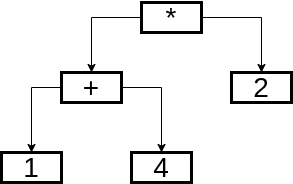
\includegraphics[width=\textwidth,height=0.82\textheight,keepaspectratio]{chapter05/imgs/tree.png}

\begin{itemize}

\item
  Par\^{e}nteses determinam a estrutura mas n\~{a}o aparecem na AST
\item
  Nós internos: operadores; folhas: literais inteiros
\end{itemize}
\end{frame}

\begin{frame}[fragile]{Tipo Haskell para a AST}
\protect\hypertarget{tipo-haskell-para-a-ast}{}
\begin{lstlisting}[language=Haskell]
data Exp
  = EInt Int        -- literal inteiro
  | Exp :+: Exp     -- adi\c{c}\~{a}o
  | Exp :*: Exp     -- multiplica\c{c}\~{a}o
\end{lstlisting}

\begin{itemize}

\item
  Um construtor por constru\c{c}\~{a}o da linguagem relevante
\item
  Construtores infixos refletem a natureza binária dos operadores
\item
  Em Haskell, é conveniente usar \textbf{tipos algébricos} para ASTs
\end{itemize}
\end{frame}

\begin{frame}{Outros Desafios na Análise Sintática}
\protect\hypertarget{outros-desafios-na-anuxe1lise-sintuxe1tica}{}
\begin{itemize}

\item
  \textbf{Indenta\c{c}\~{a}o significativa} (Python, Haskell): o lexer insere
  tokens de indenta\c{c}\~{a}o/desindenta\c{c}\~{a}o.
\end{itemize}
\end{frame}

\begin{frame}[fragile]{Outros Desafios na Análise Sintática}
\protect\hypertarget{outros-desafios-na-anuxe1lise-sintuxe1tica-1}{}
\begin{itemize}

\item
  \textbf{Identificadores dependentes de contexto} (C++):
  \texttt{HashTable<K,V> x;} pode ser ambíguo

  \begin{itemize}

  \item
    Depende se \texttt{HashTable} é um tipo ou uma
    variável
  \item
    Requer feedback do analisador sem\^{a}ntico para o léxico
  \end{itemize}
\end{itemize}
\end{frame}

\hypertarget{conclusuxe3o}{%
\section{Conclus\~{a}o}\label{conclusuxe3o}}

\begin{frame}{Conclus\~{a}o}
\protect\hypertarget{conclusuxe3o-1}{}
\begin{itemize}

\item
  \textbf{GLCs} permitem especificar estruturas recursivas que ERs n\~{a}o
  conseguem
\item
  \textbf{Deriva\c{c}\~{o}es} mostram como strings s\~{a}o geradas pela gramática
\end{itemize}
\end{frame}

\begin{frame}{Conclus\~{a}o}
\protect\hypertarget{conclusuxe3o-2}{}
\begin{itemize}

\item
  \textbf{Ambiguidade} é resolvida com hierarquias de preced\^{e}ncia e
  associatividade
\item
  \textbf{Remo\c{c}\~{a}o de recurs\~{a}o \`{a} esquerda}: prepara a gramática para
  parsers descendentes.
\end{itemize}
\end{frame}

\begin{frame}{Conclus\~{a}o}
\protect\hypertarget{conclusuxe3o-3}{}
\begin{itemize}

\item
  \textbf{Fatora\c{c}\~{a}o \`{a} esquerda}: elimina ambiguidades de escolha com 1
  lookahead
\item
  \textbf{ASTs}: representa\c{c}\~{a}o compacta do programa para fases seguintes
\end{itemize}
\end{frame}
